
\section{High Speed Serial Interface Integration with Partitioned NoC}
\subsection{Block Schematic}
\begin{frame}
\frametitle{Aurora 8B10B Xilinx IP Core}
This shows a simplified block schematic of Aurora IP Core generated using Xilinx CoreGen.\\
	\centering
	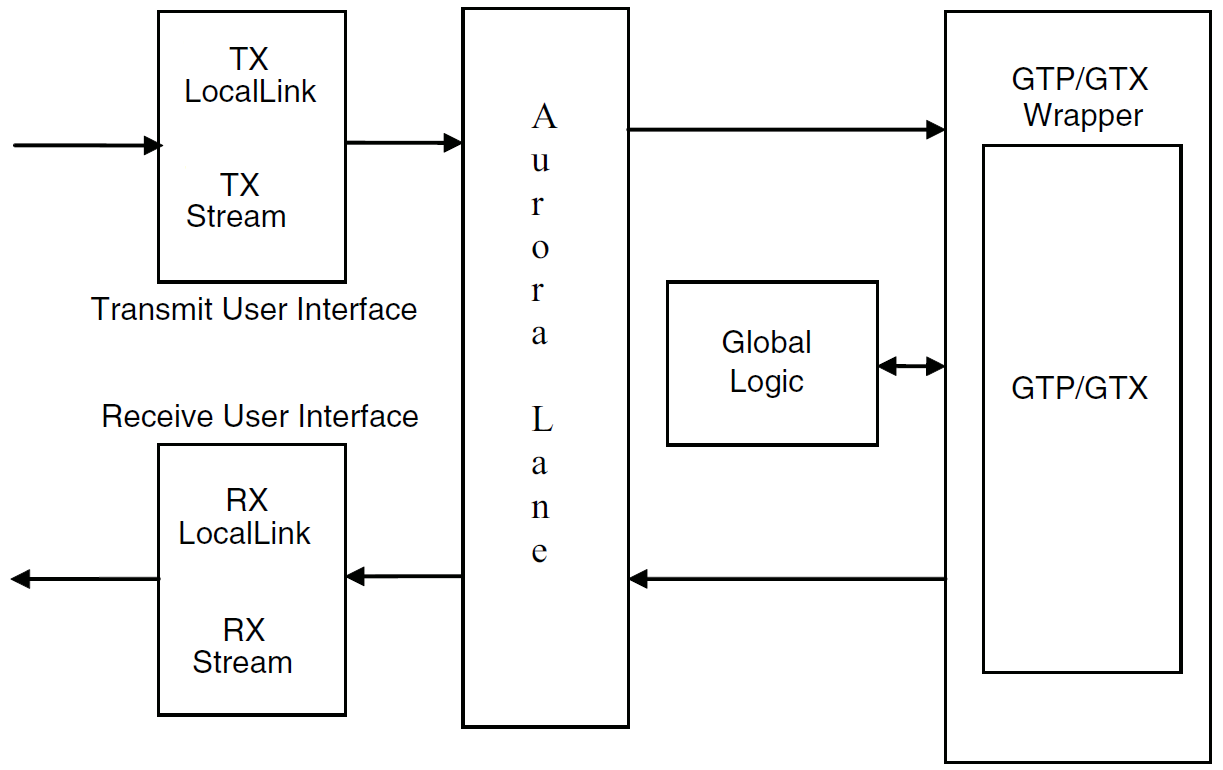
\includegraphics[scale=0.2]{./figs/auroraTop}
\end{frame}

\subsection{Experimental Setup}
\begin{frame}
\frametitle{Experimental Setup}
The figure shown below is and experimental setup of partitioned NoC integrated with Aurora core.\\
	\centering
	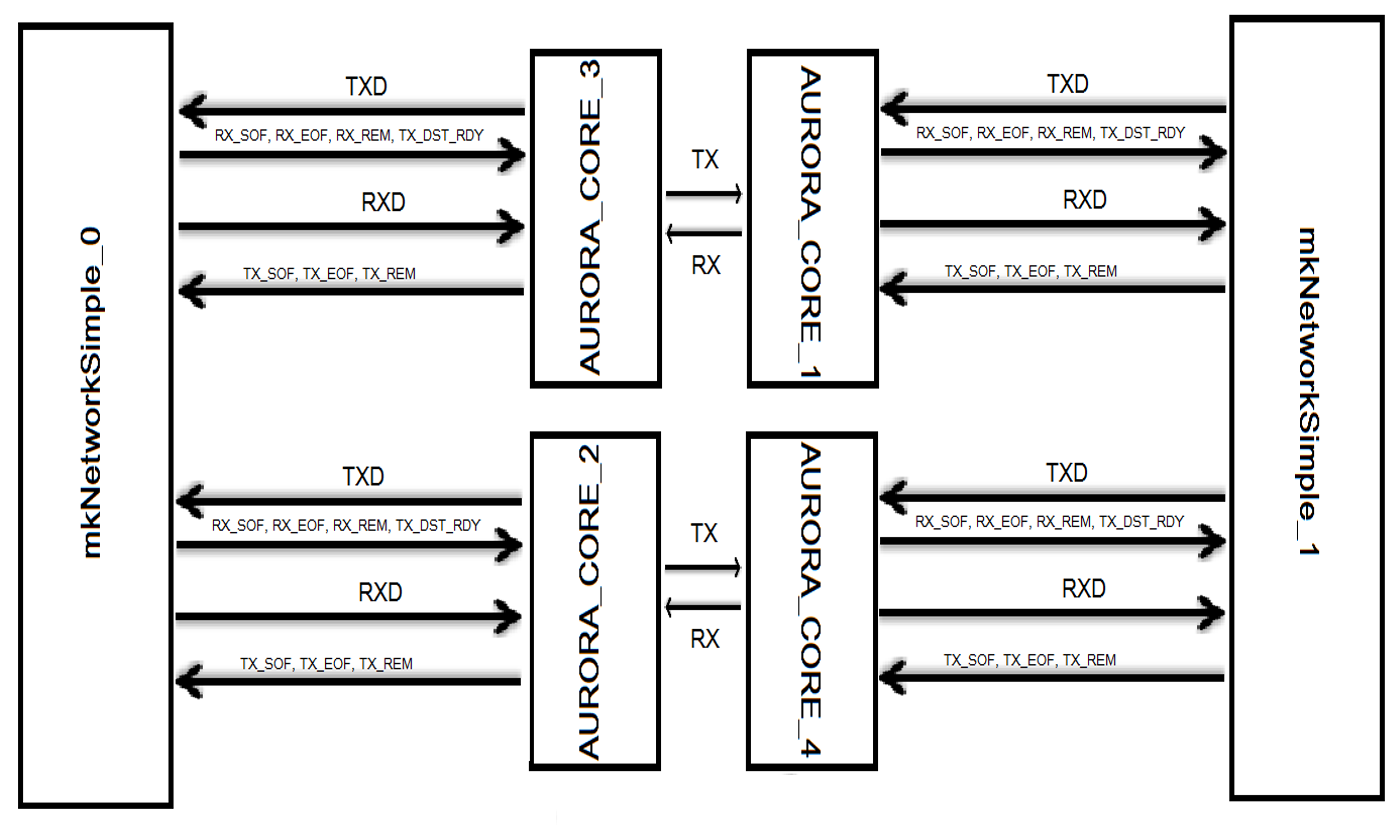
\includegraphics[scale=0.2]{./figs/PartitioningArchitecture}
\end{frame}

\subsection{Simulation Result}
\begin{frame}
\frametitle{Simulation Result}
\begin{itemize}
\item Simulation results shows a latency of 36 clock cycles
\item Here the system clock and Aurora clocks are different
\item System is running at 156.25 MHz 
\item The data rates obtained is 3.125Gbps \\
i.e. each 16 bit data (encoded to 20 bits using 8B10B encoding) is transferred is single system clock \\
Therefore, effective giving data rate of \\
\centering
156.25 MHz $\times$ 16 = 2.5Gbps or \\
156.25 MHz $\times$ 20 = 3.125 Gbps
\end{itemize}
\end{frame}

\begin{frame}
\frametitle{Simulation Result}
	\centering
	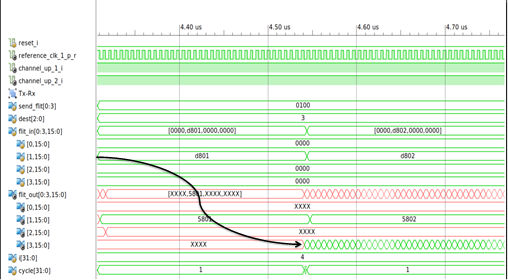
\includegraphics[scale=0.7]{./figs/AuroraSimulation}
\end{frame}

\subsection{Advantages and Disadvantages}
\begin{frame}
\frametitle{Advantages and Disadvantages}
\begin{itemize}
\item{Easy Core generation and available example design helps integrating user application}
\item{User flow control (UFC) allows applications to send a brief, high-priority message through the Aurora 8B/10B channel.}
\item{Very high data rates can be obtained ideally 3.125Gbps}
\item{Aurora core uses Gigabyte Transceiver Pair (GTP) for high speed serial interface between partitioned NoC which can be a limitation}
\item{This core is device and vendor specific which limits the user}
\end{itemize}
\end{frame}


